\chapter{Bitcoin}
\section{Introduzione}
Il Bitcoin non è propriamente una moneta, ma un sistema di pagamento. Sfrutta i protocolli crittografici per due aspetti:
\begin{itemize}
	\item generare nuova moneta
	\item attestare il possesso della valuta da parte degli utenti.
\end{itemize} 
Nel compiere una transazione è necessario indicare una chiave privata: è l'unica cosa che permette di accertare il possesso dei Bitcoin, perdere la chiave significa perdere i Bitcoin. 
\paragraph{Nascita} Nasce nel 2008 con la pubblicazione di \emph{Bitcoin: a peer to peer Electronic cash system} a cura di \emph{Satoshi Nakamoto} (pseudonimo per una persona o un gruppo ancora ignoto).
\begin{itemize}
	\item Nel 2009 viene rilasciato il primo software per partecipare (bitcoin-core) ed il 3 Gennaio 2009 viene creato il \emph{blocco genesi}. 
	\item Il 12 Gennaio 2009 avviene la prima transazione: Satoshi Nakamoto invia 10 Bitcoin ad Hal Finney (il creatore del proof of work).
	\item Nel 2010 avviene la prima transazione commerciale: vengono pagate due pizze.
\end{itemize}

\paragraph{Caratteristiche} 
\begin{itemize}
	\item Questo sistema distribuito è caratterizzato da un libro contabile (\emph{ledger}) pubblico e distribuito costituito da singoli blocchi concatenati tra di loro: la \emph{blockchain}.
	\item La \textbf{blockchain} è una lista di blocchi contenenti centinaia di transazioni: si parla di catena perchè ogni blocco è legato ai precedenti tramite il calcolo di una funzione hash. 
	\item \textbf{Il primo blocco}. Il blocco genesi è il primo blocco di questa catena: con questo si sono creati i primi 50 bitcoin.
	\item \textbf{Numero di bitcoin generati con la creazione di un nuovo blocco}.
	
	Ogni volta che si riesce ad aggiungere un nuovo blocco si creano nuovi bitcoin ed ogni 4 anni circa si dimezza la moneta generata (inizialmente 50 bitcoin per blocco, ora 6.25 per blocco).
	\item \textbf{Deadline per la creazione di Bitcoin}. 
	
	La generazione ha un tempo massimo infatti nel 2140 l'aggiunta di blocchi non genererà più nuova moneta.
\end{itemize}

\section{Funzionamento}
Dopo aver scaricato il software necessario l'utente genera una sua coppia di chiavi
$$<K_A[\text{pub}], K_A[\text{priv}]>$$
\begin{itemize}
    \item \textbf{Chiave pubblica} $K_A[\text{pub}]$: costituisce l'indirizzo identificativo dell'utente, si usa per ricevere Bitcoin e \textbf{\underline{per verificare la firma}}
    \item \textbf{Chiave privata} $K_A[\text{priv}]$: si usa per firmare le transazioni (quindi per spendere)
\end{itemize}
Il tutto si basa sulla \textbf{crittografia a curve ellittiche}. 

\paragraph{Attenzione} Nel caso in cui venga persa la chiave privata non potremo più porci come legittimi proprietari del Bitcoin. Chiunque individui la chiave privata può porsi in modo legittimo come proprietario.

\paragraph{Wallet} Il \emph{wallet} è l' insieme delle credenziali che attestano la proprietà dei BTC: la coppia indirizzo/chiave privata. Ogni utente, nel software di gestione, ha un suo Wallet.

\subsection{Transazione}
La transizione è lo scambio di valuta tra due utenti. Immaginiamo che Alice voglia inviare un numero di $x$ BTC a Bob, il messaggio avrà la forma $m$ e verrà corredato da \emph{hash} e \emph{firma}
\begin{align*}
	m &= {\text{address}}_A - x - {\text{address}}_B\\
	h &= SHA_{256}(m)\\
	f &= D(h, K_A[priv])
\end{align*}
Nel compiere la transizione verrà diffusa in rete (rete peer-to-peer, comunicazione di tipo broadcast) la coppia $<m, f>$\footnote{Attenzione al refuso sul libro, si trasmette $f$ e non $h$.}.
\paragraph{Attesa} Essendo su un sistema distribuito il destinatario deve aspettare che la rete convalidi la transazione e richiede almeno 10 minuti.
\paragraph{Molteplicità dei rami di blockchain} Dopo 10 minuti il blocco verrà aggiunto alla blockchain, bisogna poi aspettare l'aggiunta di altri 6 blocchi al nostro ramo per essere sicuri al 100\% di aver compiuto una transazione: questo perchè sulla catena di blockchain si formano vari rami. Il ramo delle transazioni considerate effettivamente valide è solo quello ufficiale: chi compie transazioni deve stare attento su questo, altrimenti le transazioni potrebbero non essere valide (in quel caso ci si trova su \emph{blocchi orfani}, chi ha pagato è come se non avesse pagato).

\section{Frazionamento delle transazioni} Il frazionamento delle transazioni è questione macchinosa.
\begin{center}
	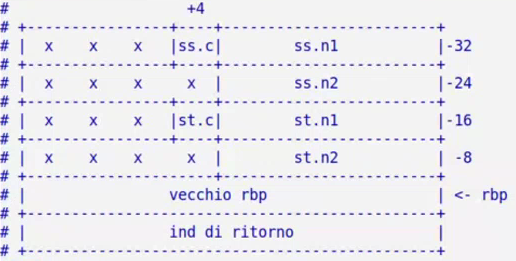
\includegraphics[width=320px]{images/31.png}
\end{center}
\subsection{Primo esempio con Bob}
Supponiamo di avere Bob che ha ricevuto 50 Bitcoin da un investitore: questi bitcoin sono l'input. Bob vuole spendere queste "monete", ma l'unica cosa che vuole fare inizialmente è trasmettere 0.5 Bitcoin ad Alice. 
\paragraph{Problema} Il patrimonio in mano a Bob è rappresentato da una o più transazioni, non è possibile scindere il contenuto di una transazione trasmettendo soltanto 0.5 Bitcoin e ignorando i rimanenti 49.5 Bitcoin. Se supponiamo i 50 Bitcoin come una banconota è come se Bob tagliasse con le forbici un pezzo di banconota. 
\paragraph{Soluzione} Nella transazione dobbiamo trasmettere tutti e 50 i Bitcoin, divideremo la cosa nel seguente modo:
\begin{itemize}
	\item 0.5 Bitcoin vanno ad Alice
	\item 49.5 vengono trasferiti a un indirizzo in mano a Bob (in un certo senso indica di volerli spedire a se stesso, potrebbe indicare la sua stessa chiave pubblica ma di solito non si fa così\footnote{Per mantenere l'anonimato}).
\end{itemize}
\subsection{Secondo esempio con Alice}
Successivamente Alice può spendere o meno i bitcoin ricevuti. Supponiamo che voglia trasmettere a un impiegato 0.8 Bitcoin. Può farlo unendo nell'input l'output di più transazione, precisamente:
\begin{itemize}
	\item 0.5 Bitcoin ricevuti prima da Bob
	\item 0.1 Bitcoin ricevuti da uno sconosciuto (ah quindi Alice parla con gli sconosciuti)
	\item 0.2 Bitcoin dalla sorella
\end{itemize}
Si possono spendere \textbf{output non spesi di precedenti transazioni} a noi destinate.

%La somma degli input deve sempre essere maggiore o uguale alla somma degli output, se è uguale pagamenti normali, se è maggiore quelli in più vengono aggiunti al primo che convalida il blocco (perché può aggiungere questo movimento).
%Per incentivare questa conferma si usa quindi lasciare questa \emph{fee} al miner.

\subsection{Validazione}
Gli utenti ricevono dal broadcast queste transazioni, le controllano (cercano nel passato se la valuta è presente nel conto di chi invia) le mettono assieme a gruppi (100, 200 anche 1000) e poi provano ad aggiungerle alla blockchain.

\paragraph{Come avviene l'aggiunta?} Ci sono vari modi per aggiungere i blocchi alla blockchain, noi vedremo il \emph{proof of work}.

\paragraph{\emph{double spending}} La blockchain previene il \emph{double spending}: per fare un paragone con la realtà è come se io pagassi due servizi diversi usando la stessa moneta, solo che al pagamento del secondo servizio i soldi non dovrebbero esserci più (sono già stati usati!). La cosa succede con la creazione di nuove transazioni nel periodo di validazione. 

\section{Struttura di un blocco della \emph{blockchain}}
Sono un nodo: arrivano le transazioni, le raggruppo in blocchi e cerco di validarle. 
\begin{center}
    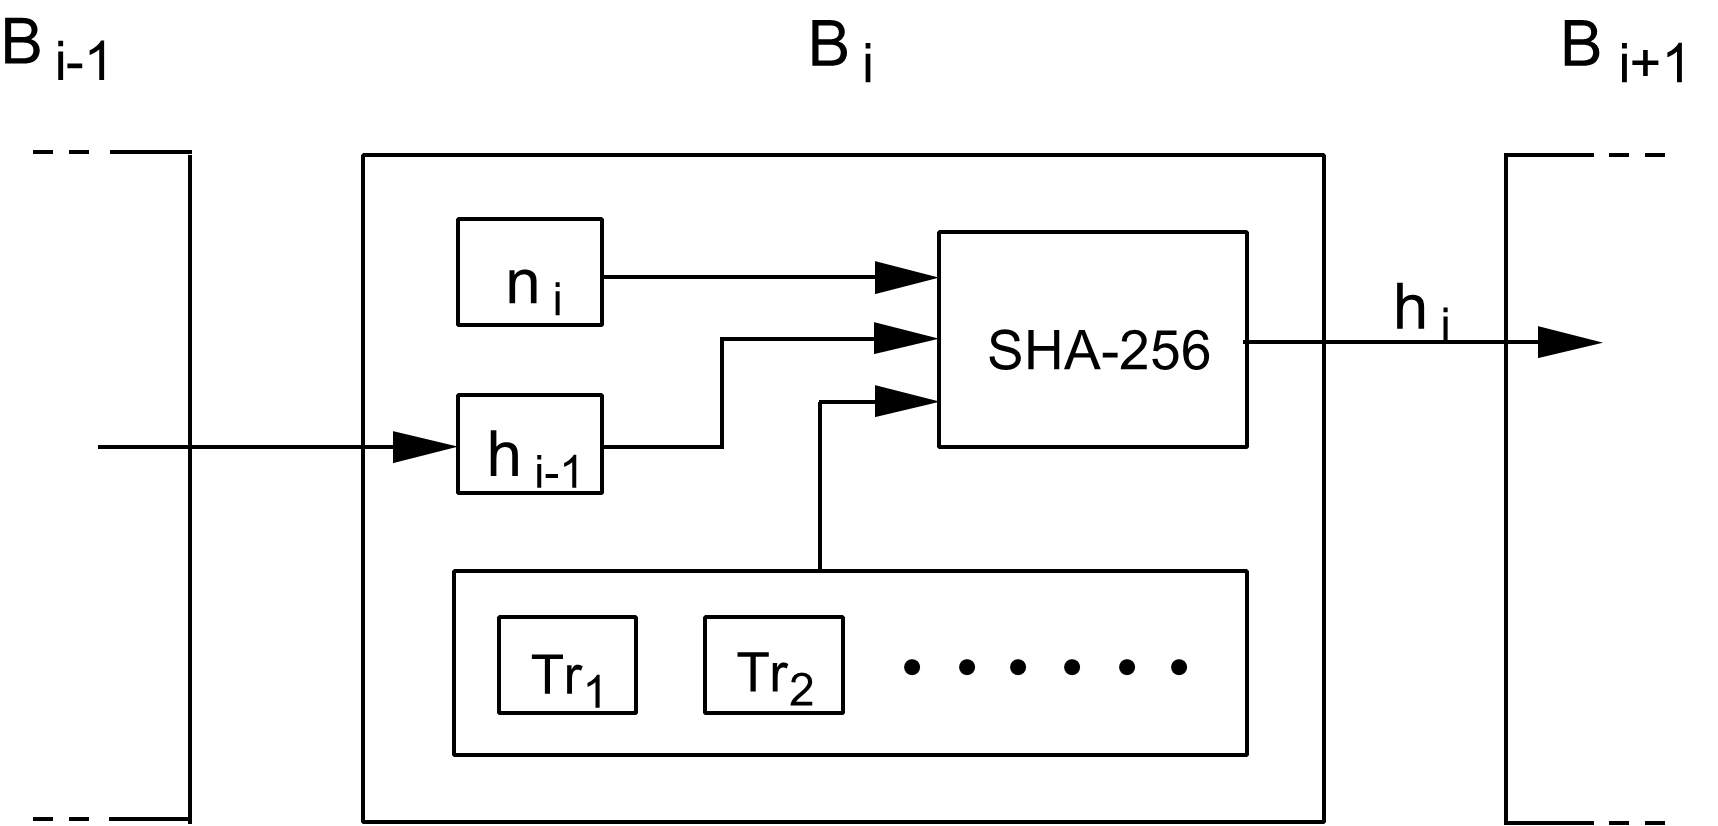
\includegraphics[width=220px]{images/Bitcoin_1.png}
\end{center}
\begin{itemize}
	\item Creo un blocco che le contiene, aggiungo la transazione finale che redirige verso di me destinatario la ricompensa.
	\item Nel blocco c'è $h_{i-1}$ cioè l'hash del blocco precedente nella catena: è importante perchè stabilisce la concatenazione col blocco precedente 
	\item Nel blocco c'è $n_i$ detto \emph{nonce}, un intero.
\end{itemize} 
Di queste informazioni faccio l'hash SHA-256 ed ottengo $h_i$, che andrà in ingresso nel blocco successivo. 
\paragraph{Richiesta} 
\begin{itemize}
	\item La richiesta è quella di ottenere un $h_i < $ di una certa soglia fissata dal sistema.
	\item Come faccio? Con una ricerca enumerativa: trovare quel valore intero $n_i$ (il \textit{nonce}) tale da soddisfare la richiesta. La richiesta è soddisfatta se troviamo un $h_i$ con $T$ zeri all'inizio.
	\item Il parametro $T$ è fissato dal sistema e varia in base alla potenza della rete.
	Questo è scelto in modo da portare il tempo di validazione di un blocco a circa 10 minuti.
	In media ci vogliono $2^T$ tentativi.
\end{itemize} 
\section{Miner e mining} Chi cerca di attaccare un nuovo blocco individuando il \textit{nonce} è detto \textbf{miner}. I miner sono i nodi che validano le transazioni aggiungendo nuovi blocchi alla blockchain. Si parla di \textbf{validazione tramite mining}.
\[\boxed{\text{La \emph{proof of work} è la ricerca del \textit{nonce}.}}\]
\begin{itemize}
	\item Cercare il \textit{nonce} è difficile
	\item Verificare il \emph{nonce} è semplice, quindi chi lo trova lo diffonde in broadcast a tutti i nodi, gli altri lo verificano, controllano la validità delle transazioni ed esprimono il loro consenso: prendono il nuovo nodo e cercheranno di attaccare nuovi nodi ad esso.
	\item Se la rete ad un certo punto ha delle biforcazioni si tende a privilegiare i rami con più transazioni perché è più probabile che siano accettati da tutta la rete.
\end{itemize}

\paragraph{Mining pool} Inizialmente Bitcoin doveva essere democratico e quindi tutti avrebbero potuto partecipare al mining, quello che è successo invece è stato che alcuni piccoli gruppi di utenti hanno unito le forze e messo a disposizione grande hardware per minare tutti assieme, ci si spartisce quindi lo spazio di ricerca del nonce e si dividono i profitti tra i vari partecipanti.

\paragraph{Aspetti sociali} Il mining ormai è poco sociale in quanto lo fanno in pochi e guadagnagno in pochi.
Inoltre si perde un sacco di energia elettrica per calcoli "inutili".
Sono state quindi sviluppate altre monete digitali che dirigono il proof work verso ambiti di ricerca per non rendere tutta questa energia elettrica sprecata

\paragraph{Attacchi alla blockchain}
Per attaccare la blockchain si deve disporre di una grande potenza di calcolo. Si possono mettere d'accordo più persone per far si che si attacchino blocchi a piacere. Si deve disporre del 51\% della rete: il che è abbastanza difficile, se avessi questa potenza però sarebbe più remunerativo giocare onestamente.












